\section{圆盘}\label{sec:圆盘}

\keyindex{圆盘}{disk}{}是一种有趣的二次曲面,
因为它有特别简单的相交例程避免求解二次方程。
pbrt中,\refvar{Disk}{}是半径为$r$沿$z$轴高度为$h$的圆盘。
它的实现在文件\href{https://github.com/mmp/pbrt-v3/tree/master/src/shapes/disk.h}{\ttfamily shapes/disk.h}和
\href{https://github.com/mmp/pbrt-v3/tree/master/src/shapes/disk.cpp}{\ttfamily shapes/disk.cpp}中。
\begin{lstlisting}
`\initcode{Disk Declarations}{=}`
class `\initvar{Disk}{}` : public `\refvar{Shape}{}` {
public:
    `\refcode{Disk Public Methods}{}`
private:
    `\refcode{Disk Private Data}{}`
};
\end{lstlisting}

为了描述部分圆盘,用户可指定最大$\varphi$值,
超出的圆盘部分被截去(\reffig{3.8})。
圆盘还能通过指定内径$r_{\mathrm{i}}$推广为\keyindex{圆环}{annulus}{}。
参数形式下,它描述为:
\begin{align*}
    \varphi & =u\varphi_{\max}\, ,                     \\
    x       & =((1-v)r+vr_{\mathrm{i}})\cos\varphi\, , \\
    y       & =((1-v)r+vr_{\mathrm{i}})\sin\varphi\, , \\
    z       & =h\, .
\end{align*}
\begin{figure}[htbp]
    \centering%LaTeX with PSTricks extensions
%%Creator: Inkscape 1.0.1 (3bc2e813f5, 2020-09-07)
%%Please note this file requires PSTricks extensions
\psset{xunit=.4pt,yunit=.4pt,runit=.4pt}
\begin{pspicture}(448.67001343,346.17999268)
{
\newrgbcolor{curcolor}{0.50196081 0.50196081 0.50196081}
\pscustom[linewidth=1,linecolor=curcolor]
{
\newpath
\moveto(247.69,221.03999268)
\curveto(247.69,215.94999268)(231.64,211.81999268)(211.84,211.81999268)
\curveto(192.04,211.81999268)(176,215.94999268)(176,221.03999268)
\curveto(176,226.12999268)(192.05,230.25999268)(211.84,230.25999268)
\curveto(222.98,230.25999268)(232.93,228.95999268)(239.5,226.90999268)
}
}
{
\newrgbcolor{curcolor}{0 0 0}
\pscustom[linewidth=1,linecolor=curcolor]
{
\newpath
\moveto(211.83000183,101.72999573)
\lineto(211.83000183,314.95999336)
}
}
{
\newrgbcolor{curcolor}{0 0 0}
\pscustom[linestyle=none,fillstyle=solid,fillcolor=curcolor]
{
\newpath
\moveto(217.34,310.04999268)
\lineto(211.83,314.30999268)
\lineto(206.33,310.04999268)
\lineto(211.83,323.05999268)
\closepath
}
}
{
\newrgbcolor{curcolor}{0.65098041 0.65098041 0.65098041}
\pscustom[linestyle=none,fillstyle=solid,fillcolor=curcolor]
{
\newpath
\moveto(216.13,311.60999268)
\lineto(211.83,321.74999268)
\lineto(211.83,314.93999268)
\closepath
}
}
{
\newrgbcolor{curcolor}{0.40000001 0.40000001 0.40000001}
\pscustom[linestyle=none,fillstyle=solid,fillcolor=curcolor]
{
\newpath
\moveto(207.53,311.60999268)
\lineto(211.83,321.74999268)
\lineto(211.83,314.93999268)
\closepath
}
}
{
\newrgbcolor{curcolor}{0 0 0}
\pscustom[linewidth=1,linecolor=curcolor]
{
\newpath
\moveto(211.83000183,102.07998657)
\lineto(132.74000549,23.97998047)
}
}
{
\newrgbcolor{curcolor}{0 0 0}
\pscustom[linestyle=none,fillstyle=solid,fillcolor=curcolor]
{
\newpath
\moveto(132.37,31.34999268)
\lineto(133.2,24.43999268)
\lineto(140.1,23.50999268)
\lineto(126.97,18.28999268)
\closepath
}
}
{
\newrgbcolor{curcolor}{0.65098041 0.65098041 0.65098041}
\pscustom[linestyle=none,fillstyle=solid,fillcolor=curcolor]
{
\newpath
\moveto(132.1,29.38999268)
\lineto(127.91,19.20999268)
\lineto(132.75,23.98999268)
\closepath
}
}
{
\newrgbcolor{curcolor}{0.40000001 0.40000001 0.40000001}
\pscustom[linestyle=none,fillstyle=solid,fillcolor=curcolor]
{
\newpath
\moveto(138.14,23.27999268)
\lineto(127.91,19.20999268)
\lineto(132.75,23.98999268)
\closepath
}
}
{
\newrgbcolor{curcolor}{0 0 0}
\pscustom[linewidth=1,linecolor=curcolor]
{
\newpath
\moveto(211.57000732,102.31999207)
\lineto(424.79998779,102.31999207)
}
}
{
\newrgbcolor{curcolor}{0 0 0}
\pscustom[linestyle=none,fillstyle=solid,fillcolor=curcolor]
{
\newpath
\moveto(419.89,96.80999268)
\lineto(424.15,102.31999268)
\lineto(419.89,107.81999268)
\lineto(432.91,102.31999268)
\closepath
}
}
{
\newrgbcolor{curcolor}{0.65098041 0.65098041 0.65098041}
\pscustom[linestyle=none,fillstyle=solid,fillcolor=curcolor]
{
\newpath
\moveto(421.45,98.01999268)
\lineto(431.59,102.31999268)
\lineto(424.78,102.31999268)
\closepath
}
}
{
\newrgbcolor{curcolor}{0.40000001 0.40000001 0.40000001}
\pscustom[linestyle=none,fillstyle=solid,fillcolor=curcolor]
{
\newpath
\moveto(421.45,106.61999268)
\lineto(431.59,102.31999268)
\lineto(424.78,102.31999268)
\closepath
}
}
{
\newrgbcolor{curcolor}{0 0 0}
\pscustom[linewidth=1,linecolor=curcolor]
{
\newpath
\moveto(350.83000183,220.86999512)
\curveto(350.83000183,229.48503133)(316.96111637,237.25183577)(265.01762877,240.5484808)
\curveto(213.07424711,243.8451191)(153.28645653,242.02232821)(113.53009079,235.93060392)
\curveto(73.77372505,229.83887963)(61.87766115,220.67781249)(83.39248224,212.71871578)
\curveto(104.90734722,204.75960284)(155.59577355,199.56999588)(211.82000732,199.56999588)
\curveto(268.0442411,199.56999588)(318.73266743,204.75960284)(340.2475324,212.71871578)
\curveto(361.7623535,220.67781249)(349.86628959,229.83887963)(310.10992386,235.93060392)
\curveto(270.35355812,242.02232821)(210.56576754,243.8451191)(158.62238587,240.5484808)
\curveto(106.67889828,237.25183577)(72.81001282,229.48503133)(72.81001282,220.86999512)
\curveto(72.81001282,212.25495891)(106.67889828,204.48815447)(158.62238587,201.19150944)
\curveto(210.56576754,197.89487113)(270.35355812,199.71766202)(310.10992386,205.80938631)
\curveto(349.86628959,211.9011106)(361.7623535,221.06217775)(340.2475324,229.02127446)
\curveto(318.73266743,236.9803874)(268.0442411,242.16999435)(211.82000732,242.16999435)
\curveto(155.59577355,242.16999435)(104.90734722,236.9803874)(83.39248224,229.02127446)
\curveto(61.87766115,221.06217775)(73.77372505,211.9011106)(113.53009079,205.80938631)
\curveto(153.28645653,199.71766202)(213.07424711,197.89487113)(265.01762877,201.19150944)
\curveto(316.96111637,204.48815447)(350.83000183,212.25495891)(350.83000183,220.86999512)
\closepath
}
}
{
\newrgbcolor{curcolor}{0 0 0}
\pscustom[linewidth=1,linecolor=curcolor]
{
\newpath
\moveto(211.74000549,221.13999176)
\lineto(291.57000732,238.28999329)
}
}
{
\newrgbcolor{curcolor}{0 0 0}
\pscustom[linewidth=1,linecolor=curcolor]
{
\newpath
\moveto(211.88999939,221.13999176)
\lineto(350.79000854,221.13999176)
}
}
{
\newrgbcolor{curcolor}{0 0 0}
\pscustom[linewidth=1,linecolor=curcolor]
{
\newpath
\moveto(68.01000214,220.62998962)
\lineto(33.52000046,220.62998962)
}
}
{
\newrgbcolor{curcolor}{0 0 0}
\pscustom[linestyle=none,fillstyle=solid,fillcolor=curcolor]
{
\newpath
\moveto(127.31612763,212.02979508)
\curveto(127.23800263,211.67823258)(127.19894013,211.63917008)(127.19894013,211.52198258)
\curveto(127.19894013,210.97510758)(127.66769013,210.81885758)(127.94112763,210.81885758)
\curveto(128.05831513,210.81885758)(128.60519013,210.89698258)(128.83956513,211.48292008)
\curveto(128.91769013,211.67823258)(129.03487763,212.49854508)(129.73800263,216.01417008)
\curveto(129.93331513,216.01417008)(130.12862763,215.97510758)(130.55831513,215.97510758)
\curveto(134.69894013,215.97510758)(138.52706513,219.88135758)(138.52706513,223.82667008)
\curveto(138.52706513,225.77979508)(137.55050263,227.26417008)(135.67550263,227.26417008)
\curveto(132.08175263,227.26417008)(130.55831513,222.42042008)(129.07394013,217.57667008)
\curveto(126.37862763,218.08448258)(124.97237763,219.45167008)(124.97237763,221.24854508)
\curveto(124.97237763,221.95167008)(125.55831513,224.68604508)(127.04269013,226.40479508)
\curveto(127.27706513,226.63917008)(127.27706513,226.67823258)(127.27706513,226.75635758)
\curveto(127.27706513,226.83448258)(127.19894013,226.99073258)(126.96456513,226.99073258)
\curveto(126.26144013,226.99073258)(124.34737763,223.35792008)(124.34737763,220.97510758)
\curveto(124.34737763,218.63135758)(125.98800263,216.83448258)(128.64425263,216.20948258)
\closepath
\moveto(130.79269013,217.42042008)
\curveto(130.55831513,217.42042008)(130.51925263,217.42042008)(130.32394013,217.45948258)
\curveto(130.01144013,217.45948258)(130.01144013,217.45948258)(130.01144013,217.53760758)
\curveto(130.01144013,217.57667008)(130.44112763,219.88135758)(130.48019013,220.23292008)
\curveto(131.26144013,223.43604508)(133.21456513,225.81885758)(135.44112763,225.81885758)
\curveto(137.15987763,225.81885758)(137.82394013,224.49073258)(137.82394013,223.27979508)
\curveto(137.82394013,220.46729508)(134.62081513,217.42042008)(130.79269013,217.42042008)
\closepath
\moveto(130.79269013,217.42042008)
}
}
{
\newrgbcolor{curcolor}{0 0 0}
\pscustom[linestyle=none,fillstyle=solid,fillcolor=curcolor]
{
\newpath
\moveto(153.72581086,217.78697434)
\curveto(153.72581086,219.31041184)(152.94456086,220.20884934)(151.10862336,220.20884934)
\curveto(149.70237336,220.20884934)(148.76487336,219.46666184)(148.29612336,218.56822434)
\curveto(147.94456086,219.81822434)(147.00706086,220.20884934)(145.75706086,220.20884934)
\curveto(144.31174836,220.20884934)(143.41331086,219.42759934)(142.90549836,218.49009934)
\lineto(142.90549836,220.20884934)
\lineto(140.32737336,220.01353684)
\lineto(140.32737336,219.38853684)
\curveto(141.49924836,219.38853684)(141.65549836,219.27134934)(141.65549836,218.41197434)
\lineto(141.65549836,213.88072434)
\curveto(141.65549836,213.13853684)(141.46018586,213.13853684)(140.32737336,213.13853684)
\lineto(140.32737336,212.51353684)
\curveto(140.36643586,212.51353684)(141.57737336,212.59166184)(142.31956086,212.59166184)
\curveto(142.94456086,212.59166184)(144.15549836,212.51353684)(144.31174836,212.51353684)
\lineto(144.31174836,213.13853684)
\curveto(143.17893586,213.13853684)(143.02268586,213.13853684)(143.02268586,213.88072434)
\lineto(143.02268586,217.04478684)
\curveto(143.02268586,218.84166184)(144.46799836,219.70103684)(145.60081086,219.70103684)
\curveto(146.81174836,219.70103684)(146.96799836,218.76353684)(146.96799836,217.86509934)
\lineto(146.96799836,213.88072434)
\curveto(146.96799836,213.13853684)(146.81174836,213.13853684)(145.67893586,213.13853684)
\lineto(145.67893586,212.51353684)
\curveto(145.71799836,212.51353684)(146.92893586,212.59166184)(147.67112336,212.59166184)
\curveto(148.29612336,212.59166184)(149.50706086,212.51353684)(149.66331086,212.51353684)
\lineto(149.66331086,213.13853684)
\curveto(148.53049836,213.13853684)(148.37424836,213.13853684)(148.37424836,213.88072434)
\lineto(148.37424836,217.04478684)
\curveto(148.37424836,218.84166184)(149.81956086,219.70103684)(150.95237336,219.70103684)
\curveto(152.16331086,219.70103684)(152.31956086,218.76353684)(152.31956086,217.86509934)
\lineto(152.31956086,213.88072434)
\curveto(152.31956086,213.13853684)(152.16331086,213.13853684)(151.03049836,213.13853684)
\lineto(151.03049836,212.51353684)
\curveto(151.06956086,212.51353684)(152.28049836,212.59166184)(153.02268586,212.59166184)
\curveto(153.64768586,212.59166184)(154.85862336,212.51353684)(155.01487336,212.51353684)
\lineto(155.01487336,213.13853684)
\curveto(153.88206086,213.13853684)(153.72581086,213.13853684)(153.72581086,213.88072434)
\closepath
\moveto(153.72581086,217.78697434)
}
}
{
\newrgbcolor{curcolor}{0 0 0}
\pscustom[linestyle=none,fillstyle=solid,fillcolor=curcolor]
{
\newpath
\moveto(163.5255774,217.20103684)
\curveto(163.5255774,218.09947434)(163.5255774,218.76353684)(162.7052649,219.42759934)
\curveto(162.0021399,220.01353684)(161.1818274,220.28697434)(160.1271399,220.28697434)
\curveto(158.4865149,220.28697434)(157.3146399,219.66197434)(157.3146399,218.60728684)
\curveto(157.3146399,218.02134934)(157.7052649,217.74791184)(158.1740149,217.74791184)
\curveto(158.6427649,217.74791184)(158.9943274,218.09947434)(158.9943274,218.56822434)
\curveto(158.9943274,218.84166184)(158.8380774,219.23228684)(158.3693274,219.34947434)
\curveto(158.9943274,219.77916184)(160.0099524,219.77916184)(160.0880774,219.77916184)
\curveto(161.0646399,219.77916184)(162.1583899,219.15416184)(162.1583899,217.66978684)
\lineto(162.1583899,217.16197434)
\curveto(161.1818274,217.12291184)(160.0490149,217.04478684)(158.7599524,216.57603684)
\curveto(157.1974524,216.02916184)(156.7287024,215.05259934)(156.7287024,214.27134934)
\curveto(156.7287024,212.78697434)(158.5255774,212.35728684)(159.7755774,212.35728684)
\curveto(161.1427649,212.35728684)(161.9630774,213.13853684)(162.3537024,213.80259934)
\curveto(162.3927649,213.09947434)(162.8615149,212.43541184)(163.6818274,212.43541184)
\curveto(163.7208899,212.43541184)(165.4005774,212.43541184)(165.4005774,214.07603684)
\lineto(165.4005774,215.05259934)
\lineto(164.8146399,215.05259934)
\lineto(164.8146399,214.11509934)
\curveto(164.8146399,213.91978684)(164.8146399,213.09947434)(164.1505774,213.09947434)
\curveto(163.5255774,213.09947434)(163.5255774,213.91978684)(163.5255774,214.11509934)
\closepath
\moveto(162.1583899,214.97447434)
\curveto(162.1583899,213.29478684)(160.6740149,212.82603684)(159.8927649,212.82603684)
\curveto(158.9943274,212.82603684)(158.1740149,213.41197434)(158.1740149,214.27134934)
\curveto(158.1740149,215.24791184)(158.9943274,216.57603684)(162.1583899,216.69322434)
\closepath
\moveto(162.1583899,214.97447434)
}
}
{
\newrgbcolor{curcolor}{0 0 0}
\pscustom[linestyle=none,fillstyle=solid,fillcolor=curcolor]
{
\newpath
\moveto(171.57952866,216.41978684)
\lineto(171.46234116,216.57603684)
\curveto(171.46234116,216.65416184)(172.59515366,217.86509934)(172.75140366,218.02134934)
\curveto(173.37640366,218.72447434)(173.96234116,219.38853684)(175.36859116,219.38853684)
\lineto(175.36859116,220.01353684)
\curveto(174.86077866,219.97447434)(174.35296616,219.93541184)(173.88421616,219.93541184)
\curveto(173.37640366,219.93541184)(172.67327866,219.97447434)(172.16546616,220.01353684)
\lineto(172.16546616,219.38853684)
\curveto(172.43890366,219.34947434)(172.51702866,219.15416184)(172.51702866,218.99791184)
\curveto(172.51702866,218.95884934)(172.51702866,218.68541184)(172.24359116,218.41197434)
\lineto(171.03265366,217.04478684)
\lineto(169.58734116,218.68541184)
\curveto(169.39202866,218.88072434)(169.39202866,218.95884934)(169.39202866,219.03697434)
\curveto(169.39202866,219.27134934)(169.62640366,219.38853684)(169.86077866,219.38853684)
\lineto(169.86077866,220.01353684)
\curveto(169.23577866,219.97447434)(168.57171616,219.93541184)(167.90765366,219.93541184)
\curveto(167.39984116,219.93541184)(166.73577866,219.97447434)(166.22796616,220.01353684)
\lineto(166.22796616,219.38853684)
\curveto(167.00921616,219.38853684)(167.47796616,219.38853684)(167.94671616,218.88072434)
\lineto(170.09515366,216.38072434)
\curveto(170.13421616,216.34166184)(170.25140366,216.22447434)(170.25140366,216.18541184)
\curveto(170.25140366,216.14634934)(168.92327866,214.70103684)(168.76702866,214.50572434)
\curveto(168.10296616,213.80259934)(167.51702866,213.17759934)(166.14984116,213.13853684)
\lineto(166.14984116,212.51353684)
\curveto(166.65765366,212.55259934)(167.04827866,212.59166184)(167.59515366,212.59166184)
\curveto(168.10296616,212.59166184)(168.80609116,212.55259934)(169.31390366,212.51353684)
\lineto(169.31390366,213.13853684)
\curveto(169.11859116,213.17759934)(168.96234116,213.29478684)(168.96234116,213.52916184)
\curveto(168.96234116,213.88072434)(169.15765366,214.11509934)(169.43109116,214.38853684)
\lineto(170.68109116,215.75572434)
\lineto(172.16546616,213.99791184)
\curveto(172.51702866,213.64634934)(172.51702866,213.60728684)(172.51702866,213.49009934)
\curveto(172.51702866,213.17759934)(172.12640366,213.13853684)(172.04827866,213.13853684)
\lineto(172.04827866,212.51353684)
\curveto(172.20452866,212.51353684)(173.45452866,212.59166184)(174.00140366,212.59166184)
\curveto(174.54827866,212.59166184)(175.13421616,212.55259934)(175.68109116,212.51353684)
\lineto(175.68109116,213.13853684)
\curveto(174.50921616,213.13853684)(174.39202866,213.25572434)(173.96234116,213.68541184)
\closepath
\moveto(171.57952866,216.41978684)
}
}
{
\newrgbcolor{curcolor}{0 0 0}
\pscustom[linestyle=none,fillstyle=solid,fillcolor=curcolor]
{
\newpath
\moveto(442.23157013,104.08531158)
\curveto(442.38782013,104.71031158)(442.97375763,107.01499908)(444.69250763,107.01499908)
\curveto(444.80969513,107.01499908)(445.43469513,107.01499908)(445.94250763,106.70249908)
\curveto(445.23938263,106.54624908)(444.77063263,105.96031158)(444.77063263,105.33531158)
\curveto(444.77063263,104.94468658)(445.04407013,104.47593658)(445.70813263,104.47593658)
\curveto(446.25500763,104.47593658)(447.03625763,104.90562408)(447.03625763,105.92124908)
\curveto(447.03625763,107.21031158)(445.59094513,107.56187408)(444.73157013,107.56187408)
\curveto(443.28625763,107.56187408)(442.42688263,106.23374908)(442.11438263,105.68687408)
\curveto(441.48938263,107.32749908)(440.16125763,107.56187408)(439.41907013,107.56187408)
\curveto(436.84094513,107.56187408)(435.39563263,104.35874908)(435.39563263,103.73374908)
\curveto(435.39563263,103.46031158)(435.66907013,103.46031158)(435.70813263,103.46031158)
\curveto(435.90344513,103.46031158)(435.98157013,103.53843658)(436.02063263,103.73374908)
\curveto(436.88000763,106.38999908)(438.52063263,107.01499908)(439.38000763,107.01499908)
\curveto(439.84875763,107.01499908)(440.70813263,106.78062408)(440.70813263,105.33531158)
\curveto(440.70813263,104.55406158)(440.27844513,102.91343658)(439.38000763,99.39781158)
\curveto(438.98938263,97.87437408)(438.09094513,96.81968658)(436.99719513,96.81968658)
\curveto(436.84094513,96.81968658)(436.29407013,96.81968658)(435.74719513,97.13218658)
\curveto(436.37219513,97.28843658)(436.91907013,97.79624908)(436.91907013,98.49937408)
\curveto(436.91907013,99.16343658)(436.37219513,99.35874908)(436.02063263,99.35874908)
\curveto(435.23938263,99.35874908)(434.65344513,98.73374908)(434.65344513,97.91343658)
\curveto(434.65344513,96.78062408)(435.86438263,96.27281158)(436.95813263,96.27281158)
\curveto(438.63782013,96.27281158)(439.53625763,98.03062408)(439.57532013,98.14781158)
\curveto(439.88782013,97.24937408)(440.78625763,96.27281158)(442.27063263,96.27281158)
\curveto(444.84875763,96.27281158)(446.25500763,99.47593658)(446.25500763,100.10093658)
\curveto(446.25500763,100.37437408)(446.05969513,100.37437408)(445.98157013,100.37437408)
\curveto(445.74719513,100.37437408)(445.70813263,100.25718658)(445.63000763,100.10093658)
\curveto(444.80969513,97.40562408)(443.13000763,96.81968658)(442.34875763,96.81968658)
\curveto(441.37219513,96.81968658)(440.98157013,97.60093658)(440.98157013,98.46031158)
\curveto(440.98157013,99.00718658)(441.09875763,99.55406158)(441.37219513,100.64781158)
\closepath
\moveto(442.23157013,104.08531158)
}
}
{
\newrgbcolor{curcolor}{0 0 0}
\pscustom[linestyle=none,fillstyle=solid,fillcolor=curcolor]
{
\newpath
\moveto(121.95743263,20.37634658)
\curveto(122.07462013,20.72790908)(122.07462013,20.76697158)(122.07462013,20.96228408)
\curveto(122.07462013,21.39197158)(121.72305763,21.62634658)(121.33243263,21.62634658)
\curveto(121.09805763,21.62634658)(120.70743263,21.47009658)(120.47305763,21.11853408)
\curveto(120.43399513,20.96228408)(120.19962013,20.22009658)(120.12149513,19.75134658)
\curveto(119.92618263,19.12634658)(119.76993263,18.42322158)(119.61368263,17.75915908)
\lineto(118.48087013,13.26697158)
\curveto(118.40274513,12.91540908)(117.30899513,11.15759658)(115.66837013,11.15759658)
\curveto(114.41837013,11.15759658)(114.14493263,12.25134658)(114.14493263,13.18884658)
\curveto(114.14493263,14.32165908)(114.57462013,15.88415908)(115.39493263,18.07165908)
\curveto(115.78555763,19.08728408)(115.90274513,19.36072158)(115.90274513,19.86853408)
\curveto(115.90274513,20.96228408)(115.12149513,21.89978408)(113.87149513,21.89978408)
\curveto(111.48868263,21.89978408)(110.59024513,18.26697158)(110.59024513,18.07165908)
\curveto(110.59024513,17.79822158)(110.82462013,17.79822158)(110.86368263,17.79822158)
\curveto(111.13712013,17.79822158)(111.13712013,17.87634658)(111.25430763,18.26697158)
\curveto(111.95743263,20.61072158)(112.93399513,21.35290908)(113.79337013,21.35290908)
\curveto(113.98868263,21.35290908)(114.41837013,21.35290908)(114.41837013,20.57165908)
\curveto(114.41837013,19.94665908)(114.14493263,19.28259658)(113.98868263,18.81384658)
\curveto(112.97305763,16.15759658)(112.54337013,14.75134658)(112.54337013,13.57947158)
\curveto(112.54337013,11.35290908)(114.10587013,10.61072158)(115.59024513,10.61072158)
\curveto(116.56680763,10.61072158)(117.38712013,11.04040908)(118.09024513,11.74353408)
\curveto(117.77774513,10.45447158)(117.46524513,9.20447158)(116.48868263,7.87634658)
\curveto(115.82462013,7.05603408)(114.88712013,6.31384658)(113.75430763,6.31384658)
\curveto(113.40274513,6.31384658)(112.26993263,6.39197158)(111.84024513,7.36853408)
\curveto(112.23087013,7.36853408)(112.58243263,7.36853408)(112.89493263,7.68103408)
\curveto(113.16837013,7.87634658)(113.40274513,8.22790908)(113.40274513,8.69665908)
\curveto(113.40274513,9.47790908)(112.73868263,9.55603408)(112.50430763,9.55603408)
\curveto(111.91837013,9.55603408)(111.09805763,9.16540908)(111.09805763,7.95447158)
\curveto(111.09805763,6.70447158)(112.19180763,5.76697158)(113.75430763,5.76697158)
\curveto(116.29337013,5.76697158)(118.87149513,8.03259658)(119.57462013,10.84509658)
\closepath
\moveto(121.95743263,20.37634658)
}
}
{
\newrgbcolor{curcolor}{0 0 0}
\pscustom[linestyle=none,fillstyle=solid,fillcolor=curcolor]
{
\newpath
\moveto(208.32254713,329.13131158)
\curveto(209.65067213,330.57662408)(210.39285963,331.20162408)(211.29129713,331.98287408)
\curveto(211.29129713,331.98287408)(212.81473463,333.31099908)(213.71317213,334.20943658)
\curveto(216.09598463,336.51412408)(216.64285963,337.72506158)(216.64285963,337.84224908)
\curveto(216.64285963,338.07662408)(216.40848463,338.07662408)(216.36942213,338.07662408)
\curveto(216.17410963,338.07662408)(216.13504713,338.03756158)(215.97879713,337.80318658)
\curveto(215.23660963,336.59224908)(214.72879713,336.20162408)(214.14285963,336.20162408)
\curveto(213.51785963,336.20162408)(213.24442213,336.59224908)(212.85379713,337.02193658)
\curveto(212.38504713,337.56881158)(211.95535963,338.07662408)(211.13504713,338.07662408)
\curveto(209.26004713,338.07662408)(208.12723463,335.77193658)(208.12723463,335.22506158)
\curveto(208.12723463,335.10787408)(208.20535963,334.95162408)(208.40067213,334.95162408)
\curveto(208.63504713,334.95162408)(208.67410963,335.06881158)(208.75223463,335.22506158)
\curveto(209.22098463,336.39693658)(210.66629713,336.39693658)(210.86160963,336.39693658)
\curveto(211.36942213,336.39693658)(211.83817213,336.24068658)(212.42410963,336.04537408)
\curveto(213.43973463,335.65474908)(213.71317213,335.65474908)(214.33817213,335.65474908)
\curveto(213.43973463,334.60006158)(211.36942213,332.80318658)(210.90067213,332.41256158)
\lineto(208.63504713,330.30318658)
\curveto(206.95535963,328.62349908)(206.05692213,327.21724908)(206.05692213,327.02193658)
\curveto(206.05692213,326.78756158)(206.33035963,326.78756158)(206.36942213,326.78756158)
\curveto(206.56473463,326.78756158)(206.60379713,326.82662408)(206.76004713,327.10006158)
\curveto(207.34598463,327.99849908)(208.08817213,328.66256158)(208.90848463,328.66256158)
\curveto(209.45535963,328.66256158)(209.72879713,328.42818658)(210.35379713,327.72506158)
\curveto(210.74442213,327.17818658)(211.21317213,326.78756158)(211.91629713,326.78756158)
\curveto(214.41629713,326.78756158)(215.86160963,329.95162408)(215.86160963,330.61568658)
\curveto(215.86160963,330.73287408)(215.74442213,330.88912408)(215.54910963,330.88912408)
\curveto(215.31473463,330.88912408)(215.27567213,330.73287408)(215.19754713,330.53756158)
\curveto(214.61160963,328.93599908)(213.01004713,328.46724908)(212.18973463,328.46724908)
\curveto(211.72098463,328.46724908)(211.25223463,328.62349908)(210.74442213,328.77974908)
\curveto(209.88504713,329.09224908)(209.49442213,329.20943658)(208.98660963,329.20943658)
\curveto(208.94754713,329.20943658)(208.55692213,329.20943658)(208.32254713,329.13131158)
\closepath
\moveto(208.32254713,329.13131158)
}
}
{
\newrgbcolor{curcolor}{0 0 0}
\pscustom[linestyle=none,fillstyle=solid,fillcolor=curcolor]
{
\newpath
\moveto(20.03559513,226.65513708)
\curveto(20.03559513,226.65513708)(20.03559513,226.92857458)(19.72309513,226.92857458)
\curveto(19.13715763,226.92857458)(17.34028263,226.73326208)(16.67622013,226.65513708)
\curveto(16.48090763,226.65513708)(16.20747013,226.61607458)(16.20747013,226.18638708)
\curveto(16.20747013,225.87388708)(16.44184513,225.87388708)(16.79340763,225.87388708)
\curveto(18.00434513,225.87388708)(18.04340763,225.71763708)(18.04340763,225.44419958)
\lineto(17.96528263,224.93638708)
\lineto(14.37153263,210.60044958)
\curveto(14.25434513,210.24888708)(14.25434513,210.20982458)(14.25434513,210.05357458)
\curveto(14.25434513,209.46763708)(14.76215763,209.35044958)(14.99653263,209.35044958)
\curveto(15.38715763,209.35044958)(15.77778263,209.66294958)(15.89497013,210.01451208)
\lineto(16.36372013,211.88951208)
\lineto(16.91059513,214.11607458)
\curveto(17.06684513,214.70201208)(17.22309513,215.24888708)(17.34028263,215.79576208)
\curveto(17.37934513,215.95201208)(17.61372013,216.77232458)(17.61372013,216.92857458)
\curveto(17.69184513,217.16294958)(18.47309513,218.53013708)(19.33247013,219.23326208)
\curveto(19.87934513,219.62388708)(20.62153263,220.09263708)(21.71528263,220.09263708)
\curveto(22.76997013,220.09263708)(23.04340763,219.23326208)(23.04340763,218.33482458)
\curveto(23.04340763,217.00669958)(22.10590763,214.27232458)(21.51997013,212.74888708)
\curveto(21.32465763,212.20201208)(21.16840763,211.88951208)(21.16840763,211.38169958)
\curveto(21.16840763,210.20982458)(22.06684513,209.35044958)(23.23872013,209.35044958)
\curveto(25.58247013,209.35044958)(26.48090763,212.98326208)(26.48090763,213.17857458)
\curveto(26.48090763,213.45201208)(26.28559513,213.45201208)(26.20747013,213.45201208)
\curveto(25.93403263,213.45201208)(25.93403263,213.37388708)(25.81684513,212.98326208)
\curveto(25.46528263,211.65513708)(24.64497013,209.89732458)(23.27778263,209.89732458)
\curveto(22.84809513,209.89732458)(22.69184513,210.13169958)(22.69184513,210.71763708)
\curveto(22.69184513,211.34263708)(22.88715763,211.92857458)(23.12153263,212.47544958)
\curveto(23.51215763,213.56919958)(24.64497013,216.53794958)(24.64497013,217.98326208)
\curveto(24.64497013,219.58482458)(23.66840763,220.63951208)(21.79340763,220.63951208)
\curveto(20.23090763,220.63951208)(19.01997013,219.85826208)(18.08247013,218.72544958)
\closepath
\moveto(20.03559513,226.65513708)
}
}
{
\newrgbcolor{curcolor}{0 0 0}
\pscustom[linestyle=none,fillstyle=solid,fillcolor=curcolor]
{
\newpath
\moveto(280.06096863,208.09705608)
\curveto(279.98284363,207.70643108)(279.82659363,207.12049358)(279.82659363,207.00330608)
\curveto(279.82659363,206.57361858)(280.17815613,206.33924358)(280.56878113,206.33924358)
\curveto(280.88128113,206.33924358)(281.31096863,206.53455608)(281.50628113,207.04236858)
\curveto(281.54534363,207.12049358)(282.36565613,210.51893108)(282.48284363,210.98768108)
\curveto(282.67815613,211.80799358)(283.14690613,213.52674358)(283.26409363,214.22986858)
\curveto(283.38128113,214.54236858)(284.08440613,215.71424358)(284.67034363,216.26111858)
\curveto(284.86565613,216.41736858)(285.60784363,217.08143108)(286.66253113,217.08143108)
\curveto(287.32659363,217.08143108)(287.67815613,216.76893108)(287.71721863,216.76893108)
\curveto(286.97503113,216.65174358)(286.42815613,216.06580608)(286.42815613,215.40174358)
\curveto(286.42815613,215.01111858)(286.70159363,214.54236858)(287.36565613,214.54236858)
\curveto(288.02971863,214.54236858)(288.73284363,215.12830608)(288.73284363,216.02674358)
\curveto(288.73284363,216.88611858)(287.95159363,217.62830608)(286.66253113,217.62830608)
\curveto(285.06096863,217.62830608)(283.96721863,216.41736858)(283.49846863,215.71424358)
\curveto(283.26409363,216.84705608)(282.36565613,217.62830608)(281.19378113,217.62830608)
\curveto(280.06096863,217.62830608)(279.59221863,216.65174358)(279.35784363,216.22205608)
\curveto(278.92815613,215.36268108)(278.61565613,213.87830608)(278.61565613,213.80018108)
\curveto(278.61565613,213.52674358)(278.85003113,213.52674358)(278.88909363,213.52674358)
\curveto(279.16253113,213.52674358)(279.16253113,213.56580608)(279.31878113,214.11268108)
\curveto(279.74846863,215.87049358)(280.25628113,217.08143108)(281.15471863,217.08143108)
\curveto(281.54534363,217.08143108)(281.89690613,216.88611858)(281.89690613,215.94861858)
\curveto(281.89690613,215.40174358)(281.81878113,215.12830608)(281.50628113,213.83924358)
\closepath
\moveto(280.06096863,208.09705608)
}
}
\end{pspicture}

    \caption{圆盘形状基本设置。圆盘半径为$r$,沿$z$轴高度为$h$。
        通过指定最大$\varphi$值和内径$r_{\mathrm{i}}$可扫掠出部分圆盘。}
    \label{fig:3.8}
\end{figure}

\reffig{3.9}是两个圆盘的渲染图像。
\begin{figure}[htbp]
    \centering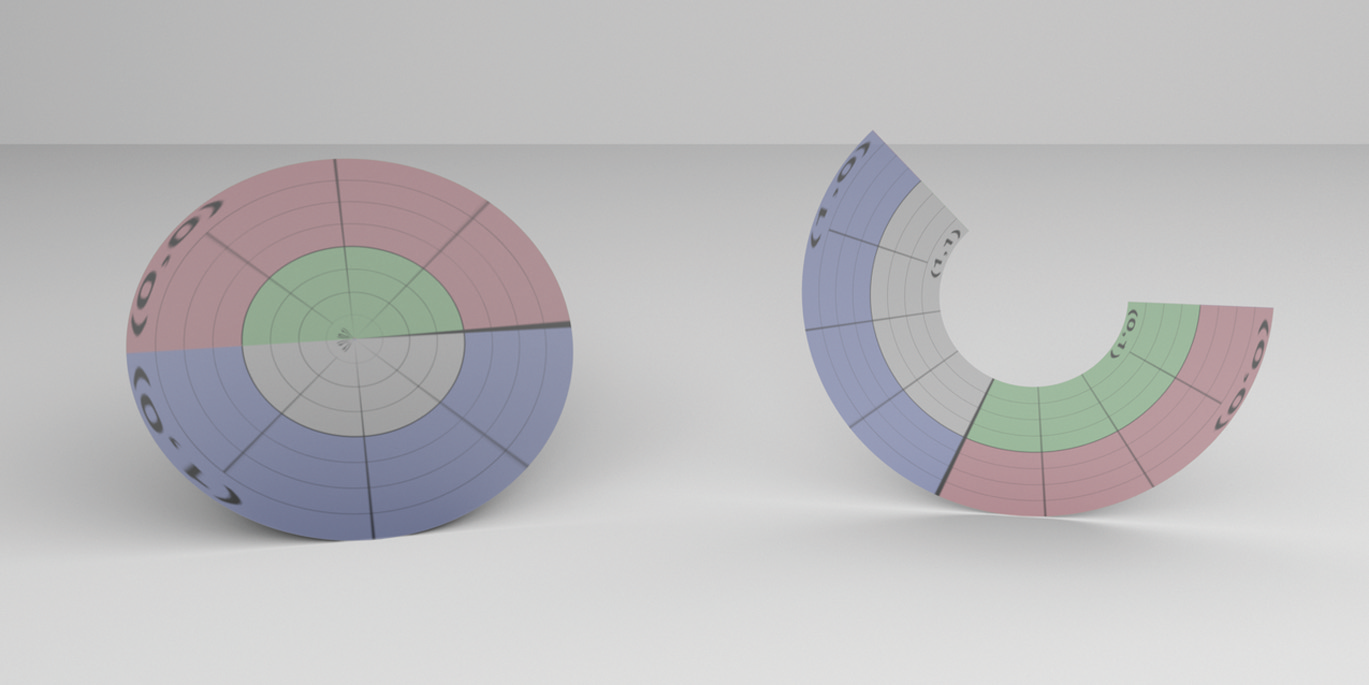
\includegraphics[width=\linewidth]{chap03/twodisks.png}
    \caption{两个圆盘。左边是完整圆盘,右边是部分圆盘。}
    \label{fig:3.9}
\end{figure}
\begin{lstlisting}
`\initcode{Disk Public Methods}{=}`
`\refvar{Disk}{}`(const `\refvar{Transform}{}` *ObjectToWorld, const `\refvar{Transform}{}` *WorldToObject,
     bool reverseOrientation, `\refvar{Float}{}` height, `\refvar{Float}{}` radius,
     `\refvar{Float}{}` innerRadius, `\refvar{Float}{}` phiMax)
    : `\refvar{Shape}{}`(ObjectToWorld, WorldToObject, reverseOrientation),
      `\refvar[Disk::height]{height}{}`(height), `\refvar[Disk::radius]{radius}{}`(radius), `\refvar[Disk::innerRadius]{innerRadius}{}`(innerRadius),
      `\refvar[Disk::phiMax]{phiMax}{}`(`\refvar{Radians}{}`(`\refvar{Clamp}{}`(phiMax, 0, 360))) { }
\end{lstlisting}
\begin{lstlisting}
`\initcode{Disk Private Data}{=}`
const `\refvar{Float}{}` `\initvar[Disk::height]{height}{}`, `\initvar[Disk::radius]{radius}{}`, `\initvar[Disk::innerRadius]{innerRadius}{}`, `\initvar[Disk::phiMax]{phiMax}{}`;
\end{lstlisting}

\subsection{边界}\label{sub:边界4}
边界方法非常简单;
它计算的边界框的中心沿$z$轴高度为$h$,
$x$和$y$方向边长都为\refvar[Disk::radius]{radius}{}。
\begin{lstlisting}
`\initcode{Disk Method Definitions}{=}\initnext{DiskMethodDefinitions}`
`\refvar{Bounds3f}{}` `\refvar{Disk}{}`::`\initvar[Disk::ObjectBound]{\refvar{ObjectBound}{}}{}`() const {
    return `\refvar{Bounds3f}{}`(`\refvar{Point3f}{}`(-`\refvar[Disk::radius]{radius}{}`, -`\refvar[Disk::radius]{radius}{}`, `\refvar[Disk::height]{height}{}`),
                    `\refvar{Point3f}{}`( `\refvar[Disk::radius]{radius}{}`,  `\refvar[Disk::radius]{radius}{}`, `\refvar[Disk::height]{height}{}`));
}
\end{lstlisting}

\subsection{相交测试}\label{sub:相交测试4}
射线与圆盘相交也很简单。射线与圆盘所在平面$z=h$相交,再检查交点是否在圆盘内。
\begin{lstlisting}
`\refcode{Disk Method Definitions}{+=}\lastnext{DiskMethodDefinitions}`
bool `\refvar{Disk}{}`::`\initvar[Disk::Intersect]{\refvar[Shape::Intersect]{Intersect}{}}{}`(const `\refvar{Ray}{}` &r, `\refvar{Float}{}` *tHit,
        `\refvar{SurfaceInteraction}{}` *isect, bool testAlphaTexture) const {
    `\refcode{Transform Ray to object space}{}`
    `\refcode{Compute plane intersection for disk}{}`
    `\refcode{See if hit point is inside disk radii and $\varphi$max}{}`
    `\refcode{Find parametric representation of disk hit}{}`
    `\refcode{Refine disk intersection point}{}`
    `\refcode{Compute error bounds for disk intersection}{}`
    `\refcode{Initialize SurfaceInteraction from parametric information}{}`
    `\refcode{Update tHit for quadric intersection}{}`
    return true;
}
\end{lstlisting}

第一步是计算射线与圆盘所在平面相交处的参数$t$值。
我们想求得射线位置$z$分量等于圆盘高度时的$t$。因此
\begin{align*}
    h=o_z+td_z\, ,
\end{align*}
即
\begin{align*}
    t=\frac{h-o_z}{d_z}\, .
\end{align*}

相交方法算出$t$值并检查它是否在合法值范围{\ttfamily (0, \refvar{tMax}{})}内。
如果不在,例程就返回{\ttfamily false}。
\begin{lstlisting}
`\initcode{Compute plane intersection for disk}{=}`
`\refcode{Reject disk intersections for rays parallel to the disk's plane}{}`
`\refvar{Float}{}` tShapeHit = (`\refvar[Disk::height]{height}{}` - ray.o.z) / ray.d.z;
if (tShapeHit <= 0 || tShapeHit >= ray.`\refvar{tMax}{}`)
    return false;
\end{lstlisting}

如果射线平行于圆盘平面(即它的$z$分量为0),则报告不相交。
射线平行于圆盘平面且在该平面内的情况有些模棱两可,
但把和圆盘边缘相交定义为“不相交”是最合理的。
必须明确处理该情况以避免下列代码生成NaN浮点值。
\begin{lstlisting}
`\initcode{Reject disk intersections for rays parallel to the disk's plane}{=}`
if (ray.d.z == 0)
    return false;
\end{lstlisting}

现在相交方法可以计算射线与平面相交的点{\ttfamily pHit}了。
知道平面相交处后,如果从命中点到圆盘中心的距离
大于\refvar{Disk::radius}{}或小于\refvar{Disk::innerRadius}{}
则返回{\ttfamily false}。
该过程可以利用中心点{\ttfamily (0,0,\refvar[Disk::height]{height}{})}的$x$和$y$坐标是零,
{\ttfamily pHit}的$z$分量等于\refvar[Disk::height]{height}{}的事实,
通过实际计算到中心的平方距离来优化。
\begin{lstlisting}
`\initcode{See if hit point is inside disk radii and $\varphi$max}{=}`
`\refvar{Point3f}{}` pHit = ray(tShapeHit);
`\refvar{Float}{}` dist2 = pHit.x * pHit.x + pHit.y * pHit.y;
if (dist2 > `\refvar[Disk::radius]{radius}{}` * `\refvar[Disk::radius]{radius}{}` || dist2 < `\refvar[Disk::innerRadius]{innerRadius}{}` * `\refvar[Disk::innerRadius]{innerRadius}{}`)
    return false;
`\refcode{Test disk $\varphi$ value against $\varphi$max}{}`
\end{lstlisting}

如果距离检查通过,则最终测试保证命中点的$\varphi$值
在零到调用者指定的$\varphi_{\max}$之间。
反解圆盘参数化得到和其他二次曲面一样的$\varphi$表达式。
\begin{lstlisting}
`\initcode{Test disk $\varphi$ value against $\varphi$max}{=}`
`\refvar{Float}{}` phi = std::atan2(pHit.y, pHit.x);
if (phi < 0) phi += 2 * `\refvar{Pi}{}`;
if (phi > `\refvar[Disk::phiMax]{phiMax}{}`)
    return false;
\end{lstlisting}

如果我们走到这一步,则与圆盘存在相交。
参数{\ttfamily u}被缩放来反映$\varphi_{\max}$指定的部分圆盘,
{\ttfamily v}通过反解参数方程算得。
命中点的偏导数方程推导过程和之前二次曲面用的一样。
因为圆盘的法线在任何地方都一样,
偏导数$\displaystyle\frac{\partial\bm n}{\partial u}$和$\displaystyle\frac{\partial\bm n}{\partial v}$都是平凡的$(0,0,0)$。
\begin{lstlisting}
`\initcode{Find parametric representation of disk hit}{=}`
`\refvar{Float}{}` u = phi / `\refvar[Disk::phiMax]{phiMax}{}`;
`\refvar{Float}{}` rHit = std::sqrt(dist2);
`\refvar{Float}{}` oneMinusV = ((rHit - `\refvar[Disk::innerRadius]{innerRadius}{}`) /
                   (`\refvar[Disk::radius]{radius}{}` - `\refvar[Disk::innerRadius]{innerRadius}{}`));
`\refvar{Float}{}` v = 1 - oneMinusV;
`\refvar{Vector3f}{}` dpdu(-`\refvar[Disk::phiMax]{phiMax}{}` * pHit.y, `\refvar[Disk::phiMax]{phiMax}{}` * pHit.x, 0);
`\refvar{Vector3f}{}` dpdv = `\refvar{Vector3f}{}`(pHit.x, pHit.y, 0.) * (`\refvar[Disk::innerRadius]{innerRadius}{}` - `\refvar[Disk::radius]{radius}{}`) /
                rHit;
`\refvar{Normal3f}{}` dndu(0, 0, 0), dndv(0, 0, 0);
\end{lstlisting}

\subsection{表面积}\label{sub:表面积4}
圆盘有计算简单的表面积,因为它们只是圆环的一部分:
\begin{align*}
    A=\frac{\varphi_{\max}}{2}(r^2-r_{\mathrm{i}}^2)\, .
\end{align*}
\begin{lstlisting}
`\refcode{Disk Method Definitions}{+=}\lastnext{DiskMethodDefinitions}`
`\refvar{Float}{}` `\refvar{Disk}{}`::`\initvar[Disk::Area]{\refvar[Shape::Area]{Area}{}}{}`() const { 
    return `\refvar[Disk::phiMax]{phiMax}{}` * 0.5 * (`\refvar[Disk::radius]{radius}{}` * `\refvar[Disk::radius]{radius}{}` - `\refvar[Disk::innerRadius]{innerRadius}{}` * `\refvar[Disk::innerRadius]{innerRadius}{}`);
}
\end{lstlisting}